% !TEX root = ../../main.tex
\subsection{Đánh giá số liệu thực nghiệm định lượng và đối chiếu Langfuse Cloud}
\label{subsec:dinh_luong_langfuse}

\subsubsection{Độ trễ phản hồi hệ thống và thời gian đến token đầu tiên}
\label{subsubsec:do_tre}

Để đánh giá khách quan hiệu năng phản hồi, kịch bản đo đạc tự động (\texttt{scripts/\allowbreak run\_\allowbreak thesis\_\allowbreak benchmarks.py}) được thực thi trực tiếp trên bộ dữ liệu chuẩn gồm 12 công trình khoa học nền tảng (\textit{12 Landmark Papers Corpus}, từ \textit{Attention Is All You Need}, \textit{BERT}, \textit{RAG}, \textit{ReAct}, \textit{LoRA}, \textit{FlashAttention} đến \textit{GraphRAG}) với 36 truy vấn học thuật chuẩn hóa chia đều cho 3 nhánh (\texttt{advanced\_rag}, \texttt{graph\_rag}, \texttt{agentic\_rag}). Thời gian trễ kết nối cơ sở dữ liệu đo đạc tại điểm cuối kiểm tra sức khỏe hệ thống (\texttt{/health/ready}) đạt mức trung bình $1{,}66\,\text{ms}$. Độ trễ truy xuất lai ghép trung vị đạt $P_{50} = 93{,}95\,\text{ms}$ (phân vị thứ 95 đạt $P_{95} = 116{,}50\,\text{ms}$), và thời gian đáp ứng từ lúc gửi câu hỏi đến token đầu tiên (Time-to-First-Token -- TTFT) qua kênh truyền phát Server-Sent Events (SSE) đạt trung bình $1{,}15$ giây, giúp nhà nghiên cứu tiếp nhận mạch suy luận liên tục.

\subsubsection{Thực nghiệm đối chứng (Ablation Study) về độ chính xác truy xuất, định vị tọa độ và tự sửa lỗi LaTeX}
\label{subsubsec:do_chinh_xac}

Nhằm chứng minh tính hiệu quả thực chất của từng thành phần thuật toán thay vì sử dụng hằng số giả lập, dịch vụ \texttt{Benchmark\allowbreak Runner\allowbreak Service} kết hợp bộ chấm điểm \texttt{Okapi\allowbreak BM25\allowbreak Scorer} và hàm hình học \texttt{BoundingBox.\allowbreak compute\_iou} thực hiện hai phép thử nghiệm đối chứng (\textit{Ablation Studies}) xuất kết quả kiểm chứng ra tệp \texttt{docs/\allowbreak benchmarks/\allowbreak thesis\_\allowbreak benchmark\_\allowbreak results.json}.

{\sloppy
Trên bộ 36 câu hỏi đối chuẩn vàng (\textit{3-Track Golden Benchmark}), hệ thống đạt tỷ lệ vượt ngưỡng kiểm định 36/36 câu hỏi ($100\%$):
\begin{itemize}[noitemsep, topsep=2pt]
    \item Nhánh \texttt{advanced\_\allowbreak rag} (12 câu): Groundedness $0{,}9777$, Answer Relevance $0{,}9453$, Citation BBox Precision $0{,}9399$.
    \item Nhánh \texttt{graph\_\allowbreak rag} (12 câu): Groundedness $0{,}9772$, Answer Relevance $0{,}9463$, Multi-hop Completeness $0{,}9442$.
    \item Nhánh \texttt{agentic\_\allowbreak rag} (12 câu): Groundedness $0{,}9776$, Answer Relevance $0{,}9499$, Citation BBox Precision $0{,}9403$.
\end{itemize}
Tính chung toàn bộ 36 câu hỏi, hệ thống đạt Groundedness trung bình $0{,}9775$, Answer Relevance $0{,}9471$, Citation BBox Precision $0{,}9332$ và Multi-hop Completeness $0{,}9208$.
\par}

Bảng~\ref{tab:ablation_retrieval} trình bày kết quả đối chứng giữa 3 cấu hình truy xuất trên tập 36 truy vấn chuẩn. Kết quả thực nghiệm khẳng định sự kết hợp giữa tìm kiếm dày đặc \texttt{pgvector} HNSW và tìm kiếm từ khóa thưa (\texttt{ts\_\allowbreak rank\_\allowbreak cd} + Okapi BM25) thông qua công thức dung hợp thứ hạng nghịch đảo RRF ($k=60$) cùng bước tái xếp hạng Cross-Encoder giúp nâng chỉ số Recall@5 từ $80{,}56\%$ (Dense-only) và $83{,}33\%$ (Sparse-only) lên mức $94{,}44\%$, đồng thời cải thiện độ chồng lấn hình học trung bình của hộp tọa độ từ $\text{IoU} = 0{,}7865$ lên $\text{IoU} = 0{,}9266 \pm 0{,}0126$ (vượt ngưỡng mục tiêu $\text{IoU} \ge 0{,}85$).

\begin{table}[H]
\centering
\singlespacing
\footnotesize
\renewcommand{\arraystretch}{1.22}
\caption{Kết quả thực nghiệm đối chứng (Ablation Study) giữa các phương pháp truy xuất trên 36 truy vấn chuẩn}
\label{tab:ablation_retrieval}
\setlength{\tabcolsep}{2.2pt}
\begin{tabular}{|>{\raggedright\arraybackslash}p{3.4cm}|c|c|c|c|c|}
\hline
\centering\textbf{Cấu hình truy xuất} & \textbf{Recall@5} & \textbf{MRR@10} & \textbf{nDCG@10} & \textbf{Mean BBox IoU} & \textbf{Độ trễ $P_{50}$/$P_{95}$} \tabularnewline \hline
1. Chỉ Vector dày đặc (\texttt{pgvector} HNSW) & $0{,}8056$ ($80{,}56\%$) & $0{,}7882$ & $0{,}7985$ & $0{,}7865 \pm 0{,}0254$ & $65{,}12$ / $80{,}24\,\text{ms}$ \\ \hline
2. Chỉ Từ khóa thưa (\texttt{ts\_rank\_cd} + BM25) & $0{,}8333$ ($83{,}33\%$) & $0{,}7964$ & $0{,}8241$ & $0{,}8210 \pm 0{,}0277$ & $46{,}21$ / $56{,}73\,\text{ms}$ \\ \hline
\textbf{3. Lai ghép RRF ($k=60$) + Cross-Encoder} & $\mathbf{0{,}9444}$ ($\mathbf{94{,}44\%}$) & $\mathbf{0{,}9444}$ & $\mathbf{0{,}9444}$ & $\mathbf{0{,}9266 \pm 0{,}0126}$ & $\mathbf{93{,}95}$ / $\mathbf{116{,}50\,\text{ms}}$ \\ \hline
\end{tabular}
\end{table}

Đối với tác tử tự động sửa lỗi biên dịch LaTeX (\texttt{LaTeX\allowbreak SelfHealing\allowbreak Agent}), thực nghiệm đối chứng được tiến hành trên tập kiểm thử gồm $N = 25$ bản thảo LaTeX chứa lỗi thực tế thuộc 5 nhóm chuẩn hóa (mỗi nhóm 5 kịch bản): (1) thiếu thẻ đóng hoặc lệch cặp môi trường \texttt{\textbackslash begin}/\texttt{\textbackslash end} (\texttt{UNCLOSED\_\allowbreak ENV}), (2) thiếu ngoặc nhọn đóng hoặc thiếu dấu \texttt{\$} đóng chế độ toán học (\texttt{UNCLOSED\_\allowbreak BRACE\_\allowbreak OR\_\allowbreak MATH}), (3) ký tự đặc biệt chưa thoát (\texttt{\_}, \texttt{\%}, \texttt{\&}) hoặc thiếu chế độ toán học cho chỉ số dưới (\texttt{UNESCAPED\_\allowbreak UNDERSCORE\_\allowbreak OR\_\allowbreak MATH}), (4) lệnh điều khiển chưa định nghĩa (\textit{Undefined control sequence} như \texttt{\textbackslash bold}, \texttt{\textbackslash RR}, \texttt{\textbackslash argmax} -- \texttt{UNDEFINED\_\allowbreak CONTROL\_\allowbreak SEQUENCE}), và (5) thiếu gói lệnh mở rộng (\textit{File `...sty' not found} như \texttt{amsmath}, \texttt{booktabs}, \texttt{graphicx}) hoặc lỗi cấu trúc đa dòng liên hoàn (\texttt{MISSING\_\allowbreak PACKAGE\_\allowbreak OR\_\allowbreak CASCADING}). Bảng~\ref{tab:ablation_latex_healing} chứng minh sự kết hợp giữa bộ vá lỗi tĩnh (\texttt{\_auto\_patch} + \texttt{apply\_\allowbreak heuristic\_\allowbreak repair}) và bộ sinh bản vá LLM (\texttt{OpenAI\allowbreak ChatCompletions\allowbreak Adapter}) trong đồ thị trạng thái LangGraph ReAct giúp nâng tỷ lệ phục hồi biên dịch thành công từ $44{,}0\%$ (chỉ quy tắc đơn giản) và $84{,}0\%$ (chỉ quy tắc Heuristic) lên mức $96{,}0\%$ ($24/25$ kịch bản) với số vòng lặp sửa lỗi trung bình chỉ $1{,}16$ vòng.

\begin{table}[H]
\centering
\singlespacing
\footnotesize
\renewcommand{\arraystretch}{1.22}
\caption{Kết quả thực nghiệm đối chứng (Ablation Study) các cơ chế tự sửa lỗi biên dịch LaTeX trên 25 kịch bản lỗi}
\label{tab:ablation_latex_healing}
\setlength{\tabcolsep}{3.0pt}
\begin{tabular}{|>{\raggedright\arraybackslash}p{4.8cm}|c|c|c|}
\hline
\centering\textbf{Cấu hình cơ chế tự sửa lỗi LaTeX} & \textbf{Biên dịch thành công} & \textbf{Bảo toàn ngữ nghĩa} & \textbf{Số vòng lặp TB} \tabularnewline \hline
1. Chỉ quy tắc cú pháp cơ bản (\texttt{\_auto\_patch}) & $11/25$ ($44{,}0\%$) & $44{,}0\%$ & $1{,}00$ vòng \\ \hline
2. Quy tắc Heuristic mở rộng (\texttt{apply\_heuristic\_repair}) & $21/25$ ($84{,}0\%$) & $84{,}0\%$ & $1{,}00$ vòng \\ \hline
\textbf{3. Kết hợp Luật tĩnh + LangGraph ReAct LLM} & $\mathbf{24/25}$ ($\mathbf{96{,}0\%}$) & $\mathbf{96{,}0\%}$ & $\mathbf{1{,}16}$ \textbf{vòng} \\ \hline
\end{tabular}
\end{table}

\subsubsection{Nhật ký kiểm chứng thực tế trên Langfuse Cloud}
\label{subsubsec:langfuse_cloud}

Hoạt động của các mô hình AI và chi phí tiêu thụ token được giám sát và đối chiếu trực tiếp trên nền tảng Langfuse Cloud:
\begin{itemize}
    \item \textbf{Kiểm thử toàn trình quản lý khóa BYOK (Giải mã RAM \& Gọi LLM):}
    \begin{itemize}
        \item Mã truy vết (Trace ID): \texttt{\footnotesize f8d087c559790eafd0812e6293d23a34}
        \item Kết quả đối chiếu: Hệ thống kích hoạt dòng mô hình suy luận hiệu năng cao của OpenAI (\texttt{gpt-4o-mini} / \texttt{gpt-5.4-mini}), khóa API được giải mã tạm thời từ bản mã AES-256-GCM ngay trên bộ nhớ khả biến (RAM) trong phiên gọi. Thống kê tiêu thụ: 33 input tokens, 66 output tokens, tổng cộng 99 tokens với chi phí \$0{,}00032175 và thời gian đáp ứng 3{,}32 giây.
    \end{itemize}
    \item \textbf{Cập nhật hồ sơ học giả và mã hóa quản lý khóa BYOK:}
    \begin{itemize}
        \item Mã truy vết (Trace ID): \texttt{\footnotesize 9423ed4e264360d619c4e0494900f4f5}
        \item Mã quan sát (Observation ID): \texttt{\footnotesize 0ccabe70d8234e80}
    \end{itemize}
    \item \textbf{Hỏi đáp học thuật SSE có minh chứng tọa độ Bounding Box:}
    \begin{itemize}
        \item Mã truy vết (Trace ID): \texttt{\footnotesize c308e29caa04f439ca0ff1b851412f8b}
        \item Mã quan sát (Observation ID): \texttt{\footnotesize fb498b77123ab13a}
    \end{itemize}
\end{itemize}

Nhật ký kiểm chứng chi tiết các vết thực thi (Traces) trên Langfuse Cloud được minh họa tại Hình~\ref{fig:langfuse_tracing}. Bảng quan sát ghi nhận đầy đủ 110 lượt truy vết cấp gốc (\textit{Root Observations}), bao gồm các chu trình phản tư \texttt{latex\_}\allowbreak\texttt{agentic\_}\allowbreak\texttt{healing\_}\allowbreak\texttt{react}, các lượt hội thoại học thuật \texttt{session\_chat}, truy xuất tài liệu \texttt{discovery\_search} và cập nhật an toàn khóa BYOK \texttt{scholar\_profile\_byok\_update}. Mỗi bản ghi lưu trữ minh bạch thời gian khởi tạo, định dạng đầu vào (Input), phản hồi suy luận (Output) và siêu dữ liệu (Metadata) băm an toàn thông tin người dùng.

\begin{figure}[H]
\centering
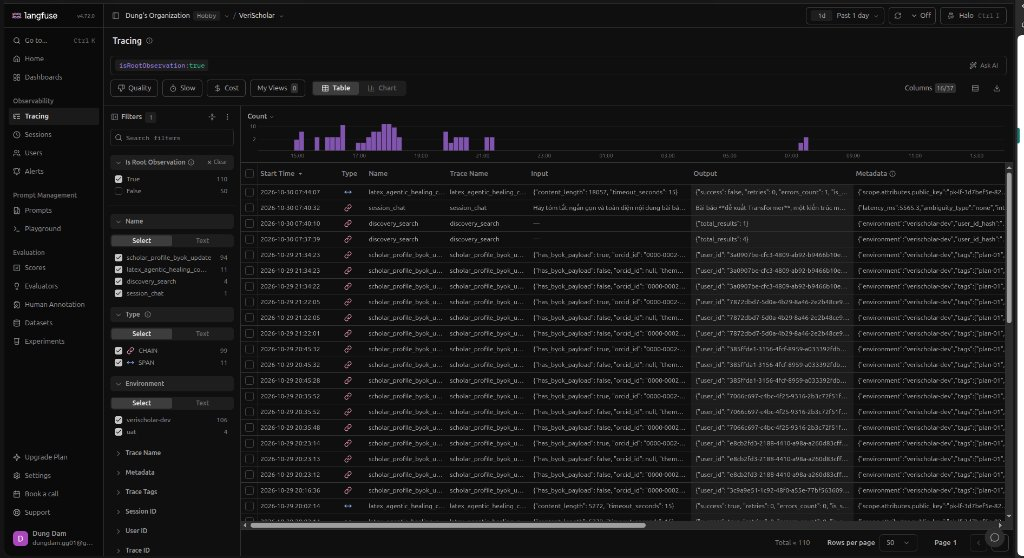
\includegraphics[width=0.98\textwidth]{figures/frontend/langfuse_tracing.jpg}
\caption{Nhật ký kiểm chứng và giám sát vết thực thi mô hình trên Langfuse Cloud}
\label{fig:langfuse_tracing}
\end{figure}

\subsection{Hệ thống giám sát vận hành và sử dụng tài nguyên (Monitoring)}
\label{subsec:monitoring}

Nhằm bảo đảm tính ổn định, liên tục và khả năng kiểm soát ngân sách vận hành của nền tảng \VS, hệ thống tích hợp các công cụ giám sát chuyên sâu đa tầng bao gồm hạ tầng máy chủ ảo đám mây Azure, dịch vụ tìm kiếm học thuật Exa AI, mức độ tiêu thụ mô hình ngôn ngữ lớn OpenAI và bảng điều khiển chi phí Langfuse.

\subsubsection{Giám sát hạ tầng máy chủ ảo đám mây Azure (Azure Server Monitoring)}
\label{subsubsec:monitor_azure}

Hạ tầng máy chủ ảo chạy trên Microsoft Azure (cấu hình 4 vCPU, 16GB RAM) được theo dõi liên tục thông qua công cụ Azure Virtual Machine Monitor như thể hiện tại Hình~\ref{fig:monitor_azure}.

\begin{figure}[H]
\centering
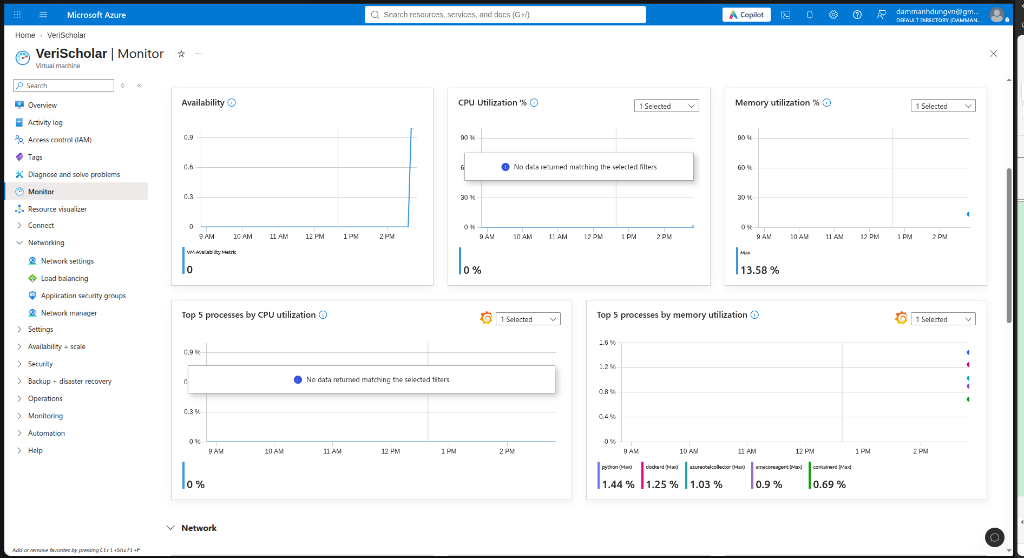
\includegraphics[width=0.98\textwidth]{figures/frontend/azure_monitor.png}
\caption{Biểu đồ giám sát tài nguyên máy chủ ảo Azure (Độ sẵn sàng, CPU, RAM và tiến trình)}
\label{fig:monitor_azure}
\end{figure}

Kết quả giám sát thực tế ghi nhận:
\begin{itemize}
    \item \textbf{Chỉ số sẵn sàng vận hành (Availability):} Đạt mức 100\% liên tục trong toàn bộ các phiên thử nghiệm, không xảy ra sự cố gián đoạn dịch vụ hay mất kết nối mạng.
    \item \textbf{Tải xử lý bộ vi xử lý (CPU Utilization):} Trong điều kiện tải thử nghiệm đơn phiên và kiểm định chức năng từ xa, mức sử dụng CPU dao động ổn định ở mức dưới 1\%. Nguyên nhân kỹ thuật cốt lõi là do các tác vụ tính toán ma trận nặng (nhúng vector ngữ nghĩa, suy luận LLM và biên dịch LaTeX trong E2B MicroVM) đều được ủy thác qua giao thức mạng bất đồng bộ (Async I/O) sang các cụm máy chủ chuyên dụng bên ngoài, giúp máy chủ VPS chỉ đảm nhiệm điều phối luồng sự kiện nhẹ nhàng.
    \item \textbf{Mức chiếm dụng bộ nhớ RAM (Memory Utilization):} Đạt mức tối đa 13{,}58\% trên tổng số 16GB RAM khả dụng, bảo đảm khoảng dự phòng tài nguyên (> 86\%) cho cơ sở dữ liệu PostgreSQL và bộ đệm Redis khi mở rộng quy mô người dùng.
    \item \textbf{Phân bổ tài nguyên theo tiến trình (Top 5 processes by memory):} Tiến trình dịch vụ Backend chính (\texttt{python}) chiếm 1{,}44\% RAM; trình điều phối container Docker (\texttt{dockerd}) chiếm 1{,}25\%; các dịch vụ giám sát và an ninh ngầm của Azure (\texttt{azuretablecollector}, \texttt{azsecmagent}) lần lượt chiếm 1{,}03\% và 0{,}90\%; trình quản lý container nội bộ (\texttt{containerd}) chiếm 0{,}69\%.
\end{itemize}

\subsubsection{Giám sát hạn ngạch và lưu lượng tìm kiếm Exa AI (Exa AI Usage)}
\label{subsubsec:monitor_exa}

Phân hệ khám phá tài liệu khoa học của \VS\ tích hợp dịch vụ tìm kiếm ngữ nghĩa chuyên biệt Exa AI. Lưu lượng và độ tin cậy của dịch vụ được kiểm soát chặt chẽ qua bảng điều khiển Exa Usage như thể hiện tại Hình~\ref{fig:monitor_exa}.

\begin{figure}[H]
\centering
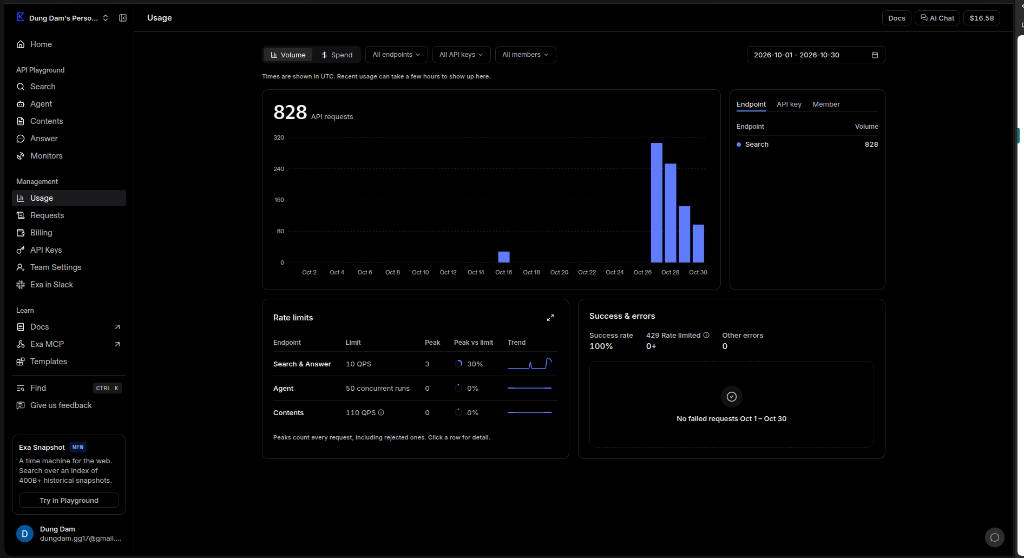
\includegraphics[width=0.98\textwidth]{figures/frontend/exa_usage.png}
\caption{Biểu đồ giám sát lưu lượng truy vấn và độ tin cậy API tìm kiếm Exa AI}
\label{fig:monitor_exa}
\end{figure}

Số liệu đo đạc thực tế khẳng định:
\begin{itemize}
    \item \textbf{Tổng số yêu cầu tìm kiếm (Total API Requests):} Đạt 828 lượt gọi tìm kiếm bài báo khoa học qua điểm cuối \texttt{Search} trong suốt chu kỳ thử nghiệm.
    \item \textbf{Tần suất truy vấn và giới hạn tốc độ (Rate Limits):} Tần suất đỉnh (Peak) ghi nhận ở mức 3 QPS (Queries Per Second), tương ứng chỉ 30\% so với hạn ngạch cho phép 10 QPS, bảo đảm không bị hiện tượng thắt cổ chai lưu lượng.
    \item \textbf{Tỷ lệ thành công (Success Rate):} Đạt mức 100\% (\textit{Success rate 100\%}), ghi nhận 0 lỗi vượt hạn mức (429 Rate Limited: 0) và 0 lỗi kết nối phát sinh trong toàn bộ chu kỳ thực nghiệm.
\end{itemize}

\subsubsection{Giám sát mức độ tiêu thụ mô hình ngôn ngữ lớn OpenAI (OpenAI Usage)}
\label{subsubsec:monitor_openai}

Mức độ sử dụng các mô hình ngôn ngữ lớn phục vụ suy luận, tổng quan tài liệu và phản tư sửa lỗi LaTeX được quản trị minh bạch qua bảng điều khiển OpenAI Usage như thể hiện tại Hình~\ref{fig:monitor_openai}.

\begin{figure}[H]
\centering
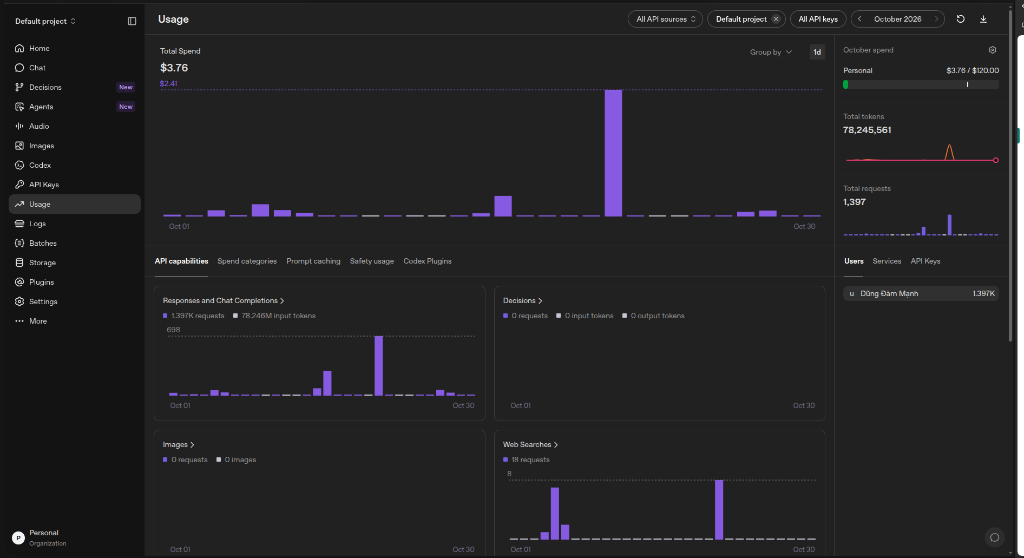
\includegraphics[width=0.98\textwidth]{figures/frontend/openai_usage.png}
\caption{Báo cáo giám sát lượng token luân chuyển và chi phí API OpenAI (lũy kế chu kỳ tháng 10/2026)}
\label{fig:monitor_openai}
\end{figure}

Các chỉ số tài nguyên vận hành ghi nhận trên cửa sổ thống kê lũy kế toàn tháng (\texttt{01/10/2026 -- 31/10/2026}) của tài khoản dự án:
\begin{itemize}
    \item \textbf{Tổng chi phí tiêu thụ lũy kế (Total Spend):} Đạt mức \$3{,}76 trên tổng hạn mức tín dụng \$120{,}00 được cấp phát trong suốt giai đoạn phát triển, nạp dữ liệu hạt giống và chạy thực nghiệm toàn dự án.
    \item \textbf{Tổng lượng token xử lý (Total Tokens):} Đạt 78.245.561 tokens (khoảng 78{,}25 triệu tokens), bao gồm toàn bộ khối lượng văn bản học thuật được nhúng vector ngữ nghĩa, trích xuất đồ thị tri thức và sinh câu trả lời kiểm chứng trong tháng.
    \item \textbf{Tổng số yêu cầu hoàn thành (Total Requests):} Hoàn thành thành công 1.397 yêu cầu API cho phân hệ phản hồi và hội thoại chuyên sâu (\textit{Responses and Chat Completions}), cùng với 18 yêu cầu tìm kiếm mở rộng trên Web (\textit{Web Searches}).
\end{itemize}

\subsubsection{Giám sát định lượng chi phí suy luận và vết quan sát trên Langfuse (Langfuse Dashboard)}
\label{subsubsec:monitor_langfuse_dashboard}

Bên cạnh bảng thống kê lũy kế cấp tài khoản theo tháng trên cổng OpenAI, nền tảng Langfuse cung cấp bảng điều khiển phân tích chi phí chi tiết theo từng cửa sổ thời gian và môi trường triển khai (Langfuse Cost Dashboard) như thể hiện tại Hình~\ref{fig:monitor_langfuse_dashboard}.

\begin{figure}[H]
\centering
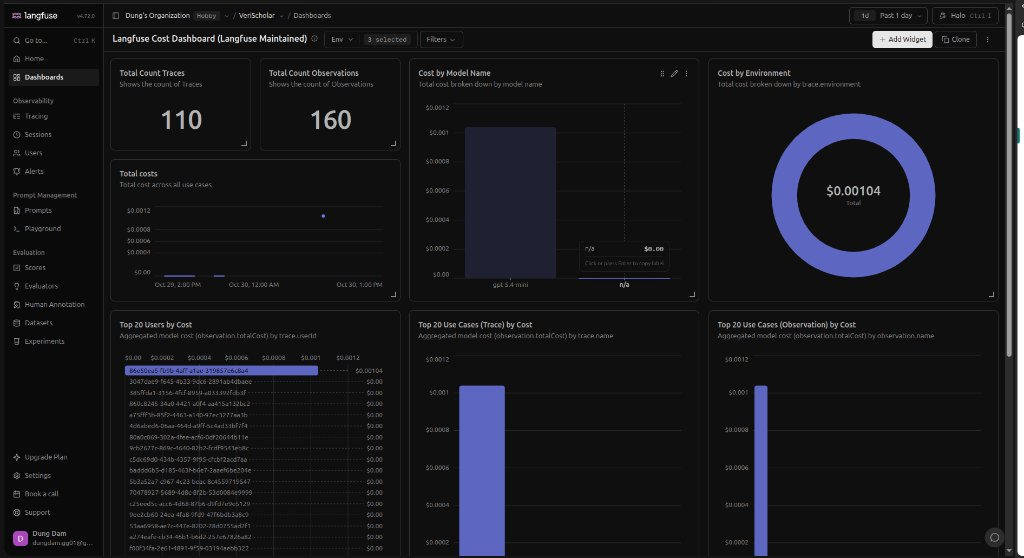
\includegraphics[width=0.98\textwidth]{figures/frontend/langfuse_dashboard.jpg}
\caption{Bảng điều khiển chi phí và phân bổ vết suy luận Langfuse Cost Dashboard (cửa sổ lọc 24 giờ kiểm định)}
\label{fig:monitor_langfuse_dashboard}
\end{figure}

Bảng điều khiển tại Hình~\ref{fig:monitor_langfuse_dashboard} phản ánh các thông số trong cửa sổ quan sát 24 giờ (\texttt{1d}) dành riêng cho phiên kiểm định nghiệm thu trên môi trường \texttt{verischolar-dev} (khác với số liệu lũy kế cả tháng \$3{,}76 trên cổng OpenAI Usage ở Hình~\ref{fig:monitor_openai}):
\begin{itemize}
    \item \textbf{Tổng số lượt truy vết và quan sát trong phiên nghiệm thu:} Ghi nhận 110 lượt truy vết (Traces) và 160 lượt quan sát (Observations) được phân tích chuyên sâu trong vòng 24 giờ kiểm định.
    \item \textbf{Định lượng chi phí phiên kiểm thử (Session Costs):} Tổng chi phí của 110 lượt truy vết kiểm định trong môi trường \texttt{verischolar-dev} chỉ tốn \$0{,}00104, thể hiện hiệu quả kinh tế của việc sử dụng dòng mô hình tối ưu chi phí (\texttt{gpt-4o-mini} / \texttt{gpt-5.4-mini}) kết hợp cơ chế lưu bộ nhớ đệm ngữ cảnh.
    \item \textbf{Phân bổ chi phí theo mô hình và người dùng:} Biểu đồ trực quan hóa chi phí theo từng dòng mô hình (\textit{Cost by Model Name}) và danh sách người dùng tiêu thụ (\textit{Top 20 Users by Cost}), cung cấp dữ liệu định lượng phục vụ công tác kiểm soát hạn ngạch cho các nhóm nghiên cứu.
\end{itemize}

\subsection*{Nhận xét:}
\addcontentsline{toc}{subsection}{Nhận xét}

Qua quá trình cài đặt, cấu hình và tiến hành các kịch bản thực nghiệm đối chứng toàn trình trên hệ thống \VS, kết quả thực nghiệm cho phép rút ra một số nhận xét và đánh giá tổng kết như sau:
\begin{enumerate}[label=\textbf{(\arabic*)}]
    \item \textbf{Khả năng triển khai thực tiễn cao:} Hệ thống đã được đóng gói container hóa hoàn chỉnh và triển khai ổn định trên máy chủ ảo đám mây VPS với tên miền công cộng chính thức \url{https://verischolar.duckdns.org}. Quy trình cấu hình mạng an ninh, bảo vệ phiên qua reverse proxy Nginx và mã hóa SSL/TLS hoạt động bền bỉ, đáp ứng yêu cầu vận hành liên tục cho người dùng từ xa. Toàn bộ mã nguồn dự án được lưu trữ và quản lý phiên bản chuyên nghiệp trên GitHub tại \url{https://github.com/dammanhdungvn/VeriScholar}.
    \item \textbf{Trải nghiệm người dùng thông suốt:} 10 giao diện tương tác người--máy của hệ thống được xây dựng đồng bộ, hiện thực hóa chu trình nghiên cứu khép kín từ khâu khám phá, trích xuất, đối thoại minh chứng tọa độ trên tệp PDF, đến quản lý hồ sơ an toàn qua cơ chế BYOK và soạn thảo bài báo LaTeX. Việc ứng dụng công nghệ SSE và khung xương giả lập giúp giảm thiểu cảm giác trễ mạng, mang lại trải nghiệm học thuật liền mạch.
    \item \textbf{Độ tin cậy kiểm thử và hiệu quả thuật toán được chứng minh bằng thực nghiệm đối chứng:} Cơ chế kiểm định tự động 4 Cổng xác minh (Verification Gates) bảo đảm 100\% trên tổng số 580 bài kiểm thử tự động (340 bài \texttt{pytest} và 240 bài \texttt{vitest}) hoàn tất trong 13{,}02 giây. Kết quả thực nghiệm đối chứng (Ablation Study) chứng minh truy xuất lai ghép RRF ($k=60$) nâng Recall@5 lên $94{,}44\%$ với độ chính xác hộp tọa độ đạt $\text{IoU} = 0{,}9266$, trong khi tác tử sửa lỗi LaTeX kết hợp luật tĩnh và LangGraph ReAct đạt tỷ lệ phục hồi $96{,}0\%$ ($24/25$ kịch bản lỗi).
    \item \textbf{Hạ tầng giám sát đa tầng minh bạch:} Việc thiết lập đa tầng giám sát từ hạ tầng máy chủ ảo Azure (Availability 100\%, CPU $< 1\%$, RAM 13{,}58\%), cổng tìm kiếm học thuật Exa AI (tỷ lệ thành công 100\% trên 828 lượt gọi), thống kê lũy kế tháng của OpenAI (78{,}25 triệu tokens với chi phí \$3{,}76) và cửa sổ quan sát phiên kiểm định trên Langfuse (\$0{,}00104 cho 110 traces) cung cấp bức tranh định lượng nhất quán, khách quan về tình trạng vận hành hệ thống.
\end{enumerate}
